\section{Durchführung}
\label{sec:Durchfuehrung}
\subsection{Aufbau der Messapparatur}
\begin{figure}
\begin{minipage}[l]{0.49\textwidth}
	\centering
	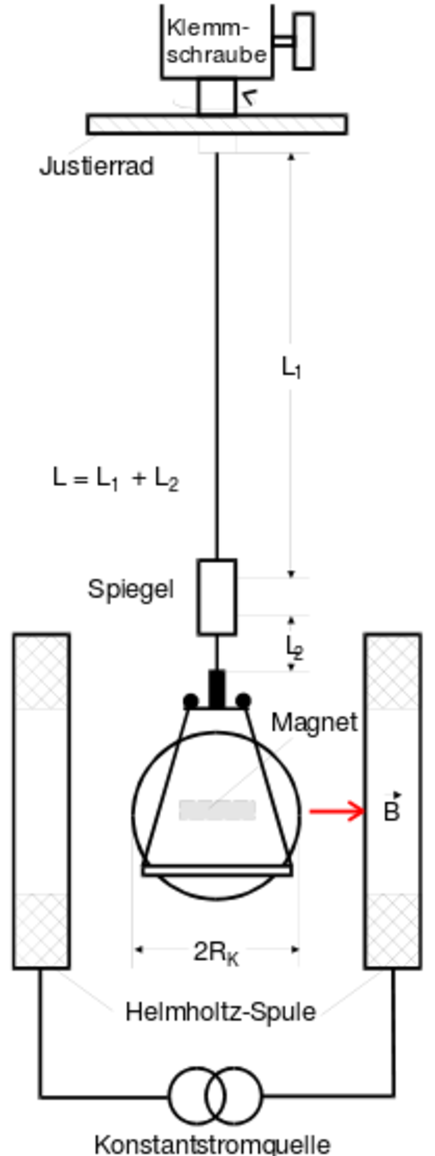
\includegraphics[width=0.4\textwidth]{Bilder/Aufbau1.pdf}
	\caption{Aufbau der Messapparatur. \cite{V102}}
	\label{fig:aufbau1}
\end{minipage}
\begin{minipage}[r]{0.49\textwidth}
	Die Periodendauer der Torsionsschwingung wird über eine elektronische Stoppuhr gemessen. 
	Mit Schwingungsbeginn soll das Zählwerk starten; nach einer Periode enden. Die Periodendauer $T$ kann dann direkt am Zählwerk abgelesen werden.
	Dieser Vorgang wird realisiert über eine, durch die in Abbildung \ref{fig:aufbau2} gezeigte Lichtschranke ,steuerbare Torstufe. 
	Das Licht einer Lampe wird zunächst durch eine Sammellinse gebündelt und anschließend durch einen Spalt auf den Spiegel am Torsionsdraht geworfen. Wird der Draht durch bewegen des Justierrades zu Schwingungen angeregt wandert der Lichtstrahl von einer Seite zur anderen und passiert dabei die Photodiode. 
	Sobald der Lichtstrahl auf die Photodiode trifft, erzeugt diese ein elektrisches Signal, welches durch eine geeignete Schaltung auf die Torsteuerungseingäng des Zählwerks geleitet wird.
\end{minipage}
\end{figure}

Abbildung \ref{fig:aufbau1} zeigt die Messapparatur. 
Am unteren Ende eines einseitig fest eingespannten Drahtes ist eine Kugel befestigt in deren Innern sich ein Permanentmagnet befindet. Sie hängt zwischen zwei Helmholtzspulen, die durch einschalten der Stromquelle ein annähernd homogenes Magnetfeld erzeugen können.
In der unteren Drahthälfte wird dieser durch einen kleinen Spiegel unterbrochen, der zur Bestimmung der Periodendauer benötigt wird.
\subsection{Messung der Schwingungsdauer}

\begin{figure}
	\centering
	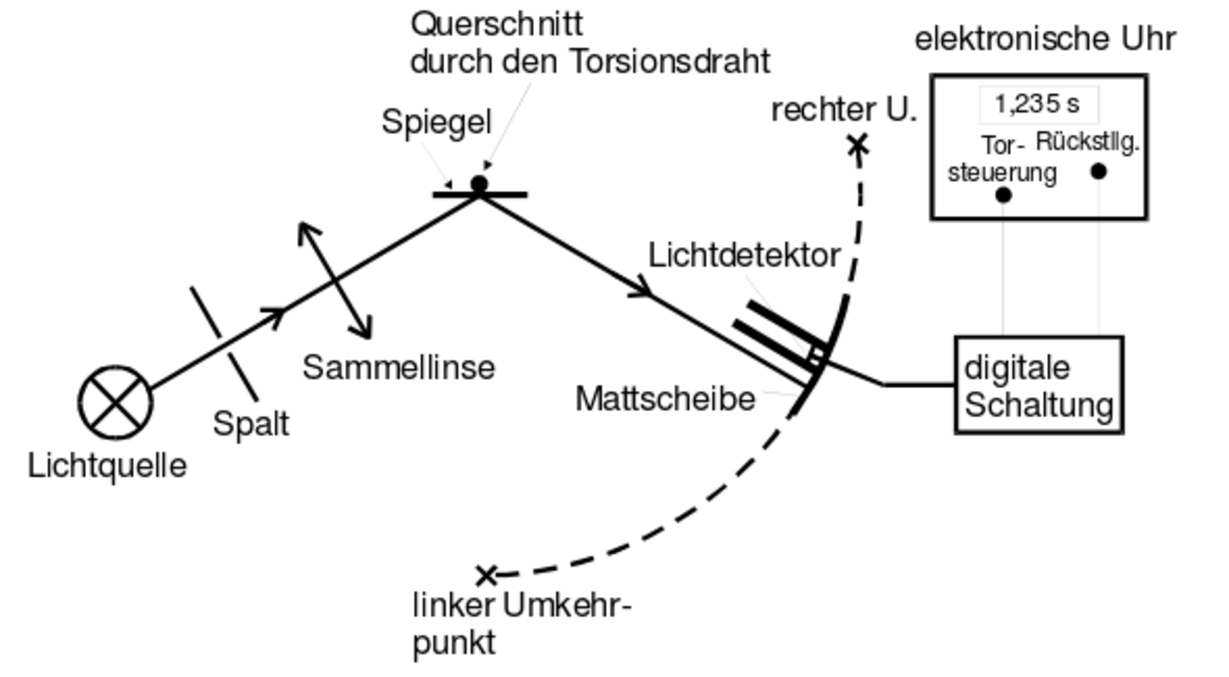
\includegraphics[width=0.7\textwidth]{Bilder/Aufbau2.pdf}
	\caption{Aufbau der Lichtschranke. \cite{V102}}
	\label{fig:aufbau2}
\end{figure}
% Die Periodendauer der Torsionsschwingung wird über eine elektronische Stoppuhr gemessen. 
% Mit Schwingungsbeginn soll das Zählwerk starten; nach einer Periode enden. Die Periodendauer $T$ kann dann direkt am Zählwerk abgelesen werden.
% Dieser Vorgang wird realisiert über eine, durch die in Abbildung \ref{fig:aufbau2} gezeigte Lichtschranke ,steuerbare Torstufe. 
% Das Licht einer Lampe wird zunächst durch eine Sammellinse gebündelt und anschließend durch einen Spalt auf den Spiegel am Torsionsdraht geworfen. Wird der Draht durch bewegen des Justierrades zu Schwingungen angeregt wandert der Lichtstrahl von einer Seite zur anderen und passiert dabei die Photodiode. 
% Sobald der Lichtstrahl auf die Photodiode trifft, erzeugt diese ein elektrisches Signal, welches durch eine geeignete Schaltung auf die Torsteuerungseingäng des Zählwerks geleitet wird.

In drei Versuchsteilen wird der Draht durch Auslenken des Justierrades zu harmonischen Schwingungen angeregt und die am Zählwerk angezeigte Schwingungsdauer notiert.

Zur Bestimmung des Schubmoduls $G$ muss der Permanentmagnet parallel zum Draht ausgerichtet sein, was der Richtung des Erdmagnetfeldes entspricht. Dieses nimmt dadurch keinen Einfluss auf die Schwingungsdauer. Es werden zehn Messwerte aufgenommen.
Anschließend wird das magnetische Moment ders Permanentmagneten bestimmt. In diesem Versuchsteil wird die Stromquelle der Helmholtz-Spulen eingeschaltet um ein Magnetfeld zu realisieren. Die Stromstärke, mit der die Spulen betrieben werden, wird von $I=0\,\si\ampere$ bis $I=1\,\si\ampere$ in fünf Schritten variiert und je fünf Schwingungsdauern notiert.
 Hier wird der Permanentmagnet senkrecht zum Draht und parallel zum Magnetfeld der Spulen ausgerichtet, um den maximalen Einfluss des Magnetfeldes  auf die Schwingung zu erreichen.  
Zur Bestimmung des Erdmagnetfelds bleibt der Permanentmagnet senkrecht zum Draht ausgerichtet, um den maximalen Einfluss des Erdmagnetfeldes auf die Schwingung zu erreichen. Erneut werden zehn Perioden gemessen.

Zur Berechnung der Module müssen außerdem Drahtlänge und -durchmesser bekannt sein. Gemessen werden diese mit einer Micrometerschraube bzw. einem Maßband.
Radius und Masse der angehängten Kugel, sowie der Befestigung, als auch Windungszahl der Spulen sind angegeben.

